\documentclass{report}
\usepackage{graphicx}
\usepackage{xcolor}
\usepackage{forest}
\usepackage{amsmath}
\usepackage{multicol}
\begin{document}
\begin{titlepage}
\begin{center}
	\vspace*{1cm}

	\Huge
	\textbf{Course Project}

	\vspace{0.5cm}
	\LARGE
	Second Deliverable: The Parser	

	\vspace{1.5cm}

	\textbf{Quin'darius Lyles-Woods}
	\Large
	qlyleswo@students.kennesaw.edu

	\vfill
	\LARGE
	Concepts of Programming Languages	\\
	Professor Jose Garrido			\\
	Section W01 				\\
	4308
	\vspace{0.8cm}

	
\includegraphics[width=\textwidth]{kennesawlogo}

	\vspace{0.8cm}

	\Large
	Bachelors of Computer Science\\
	Kennesaw State University\\
	1100 South Marietta Pkwy SE\\
	Marietta, GA 30060\\
	\today	

	\vspace{1cm}

\end{center}
\end{titlepage}


\section*{Task}
The development of an interpreter for a subset of \textbf{Basic Language}. 

\vspace{0.5cm}

\subsection*{Project Goals}
\begin{itemize}
	\item Process a \textbf{Basic Language} source code file. 
	\item Tokenize the source code file. 
	\item Detect syntactical error.
	\item Display appropriate error messages during runtime. 
\end{itemize}

\subsection*{Deliverable Goals}
\begin{itemize}
	\item Develop a grammar for the subset of \textbf{Basic Language} that I will be using. 
	\item Arrays for the \emph{Keywords} and \emph{Identifiers}
	\item Ability to input source code to lexer. 
	\item Output tokens scanned. 
\end{itemize}

\subsection*{Subset of the Basic Language}
The subset of basic that I want to define for the course project is going to be kept as minimal as possible to focus on the process of developing an interpreter. 
With that in mind the lowest we can go is turing complete of course. 
For this to be true the language doesn't need much. 

\begin{multicols}{2}
\begin{itemize}
	\item Recursive Operators
		\begin{itemize}
			\item \texttt{FOR...TO...NEXT}
		\end{itemize}
	\item Conditional Jumps 
		\begin{itemize}
			\item \texttt{IF...THEN...\{ELSE\}}
			\item \texttt{GOTO}
		\end{itemize}	
	\item Variables
		\begin{itemize}
			\item \texttt{LET}
		\end{itemize}
\end{itemize}
\columnbreak
\subsection*{Tokens}
\begin{itemize}
	\item LET
	\item IF 
	\item FOR 
	\item GOTO
	\item +
	\item -
	\item *
	\item /
	\item =
\end{itemize}

\end{multicols}
\subsection*{Backus Normal Form of Basic Subset}
\begin{align*}
BASIC \; PROGRAM &::=				\\ 
	&|\; EXPRESSION, EXPRESSION 		\\
	&|\; EXPRESSION				\\
	EXPRESSION &::=				\\
	&|\; LET				\\
	&|\; IF					\\
	&|\; FOR 				\\
	&|\; GOTO				\\
	&|\; IDENTIFIER\;+\;EXPRESSION		\\
	&|\; IDENTIFIER\;-\;EXPRESSION		\\
	&|\; IDENTIFIER\;*\;EXPRESSION		\\
	&|\; IDENTIFIER\;/\;EXPRESSION		\\
	LET &::=				\\
	&| IDENTIFIER = EXPRESSION		\\
	IDENTIFIER &::=				\\
	&|\; [a-zA-Z] 				\\
	&|\; [a-zA-Z],[a-zA-Z]			\\
	IF &::=					\\
	&|\; EXPRESSION\;then\;STATEMENT	\\
	&|\; EXPRESSION\;then\;STATEMENT\;else\;IF\\
	FOR &::=				\\
	&|\;EXPRESSION\;to\;EXPRESSION\;STATEMENT\;next\\
	GOTO &::=				\\
	&|\; [0-9] 				\\
	&|\; [0-9],[0-9] 			\\
\end{align*}

\subsection*{Source Code}
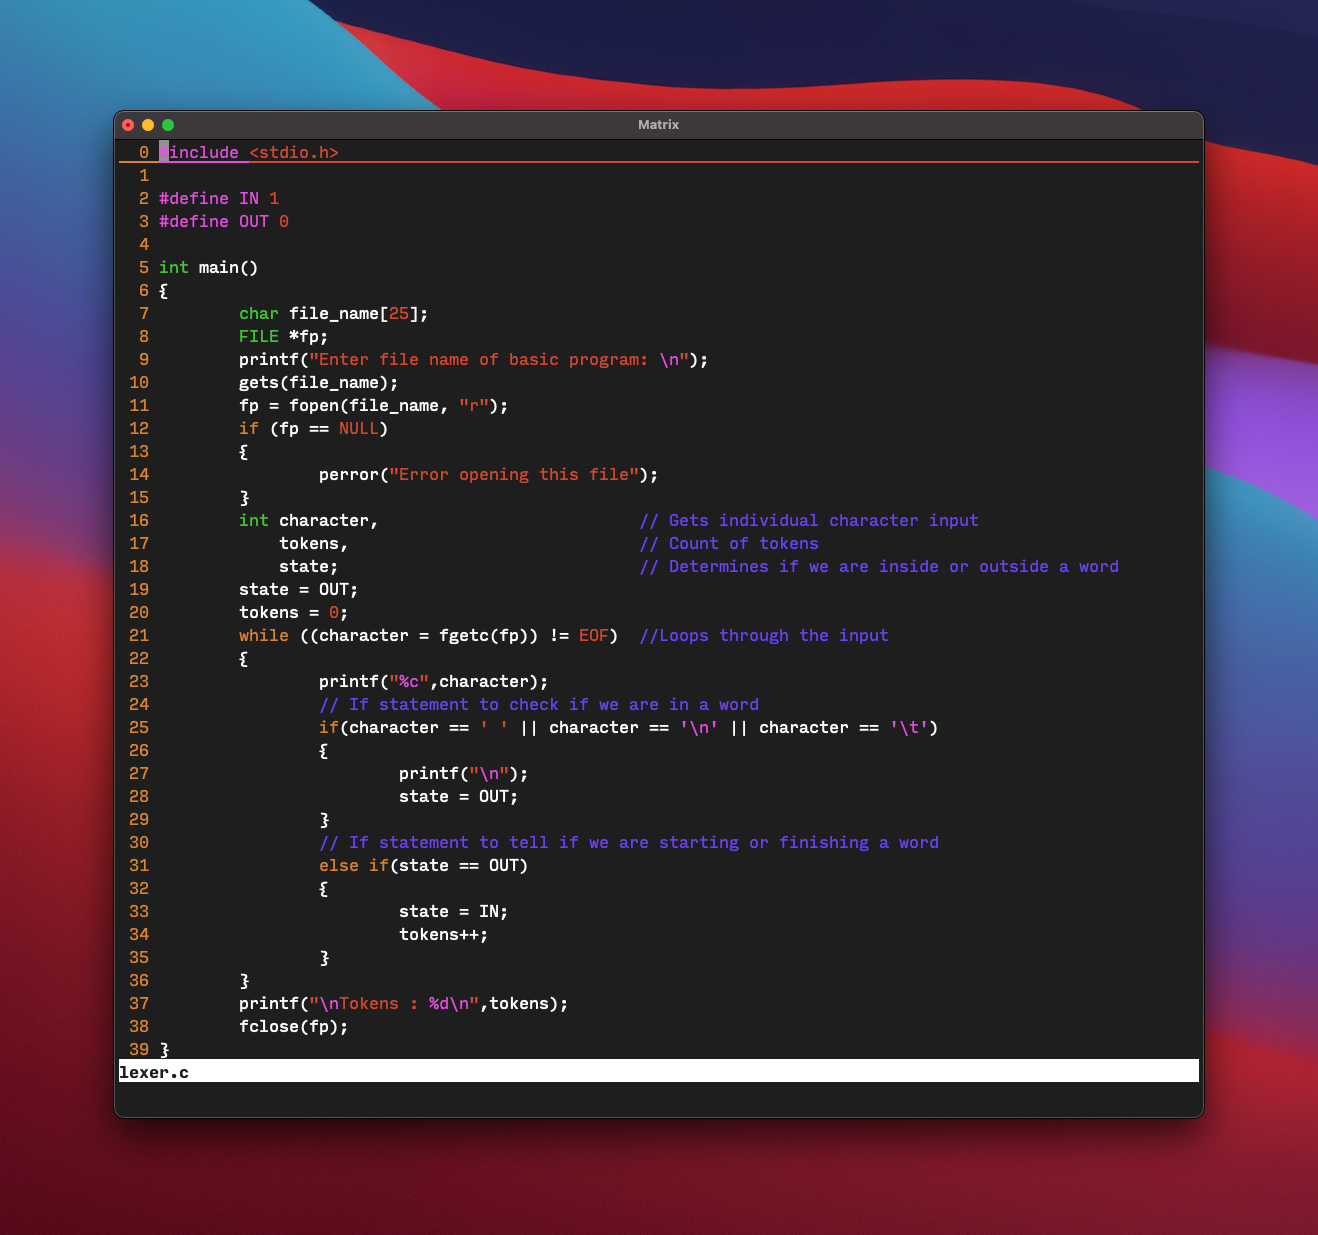
\includegraphics[width =\textwidth]{source_code}
\subsection*{Compiling}
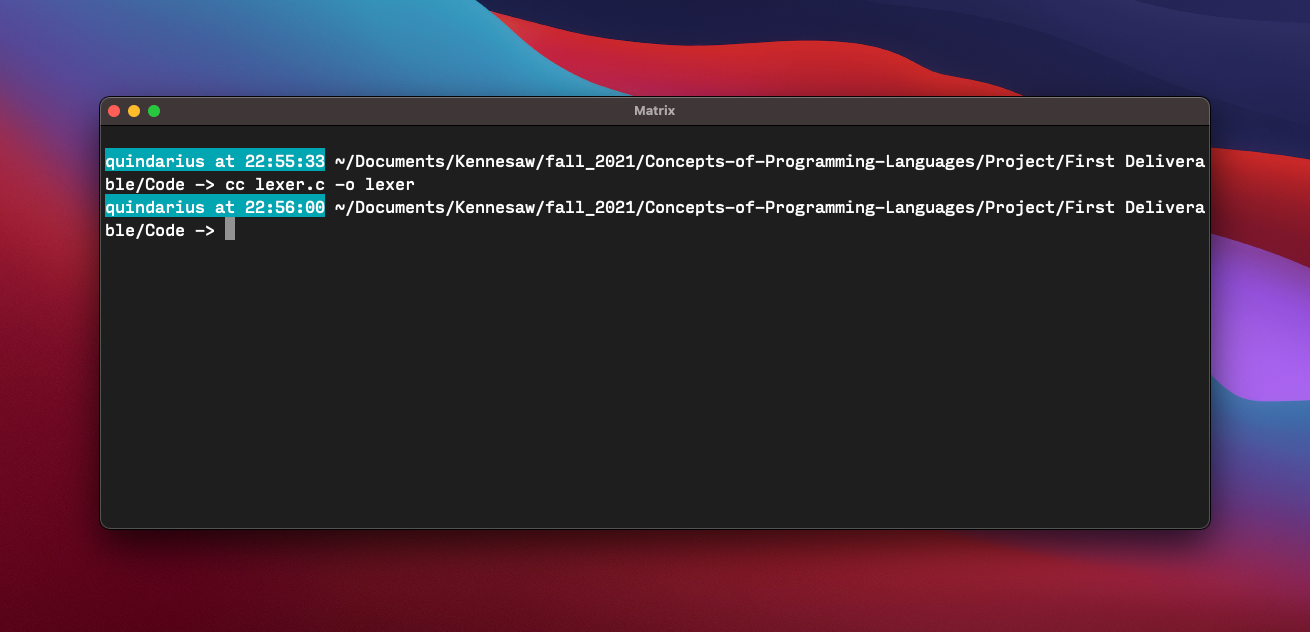
\includegraphics[width =\textwidth]{compile}
\subsection*{Output}
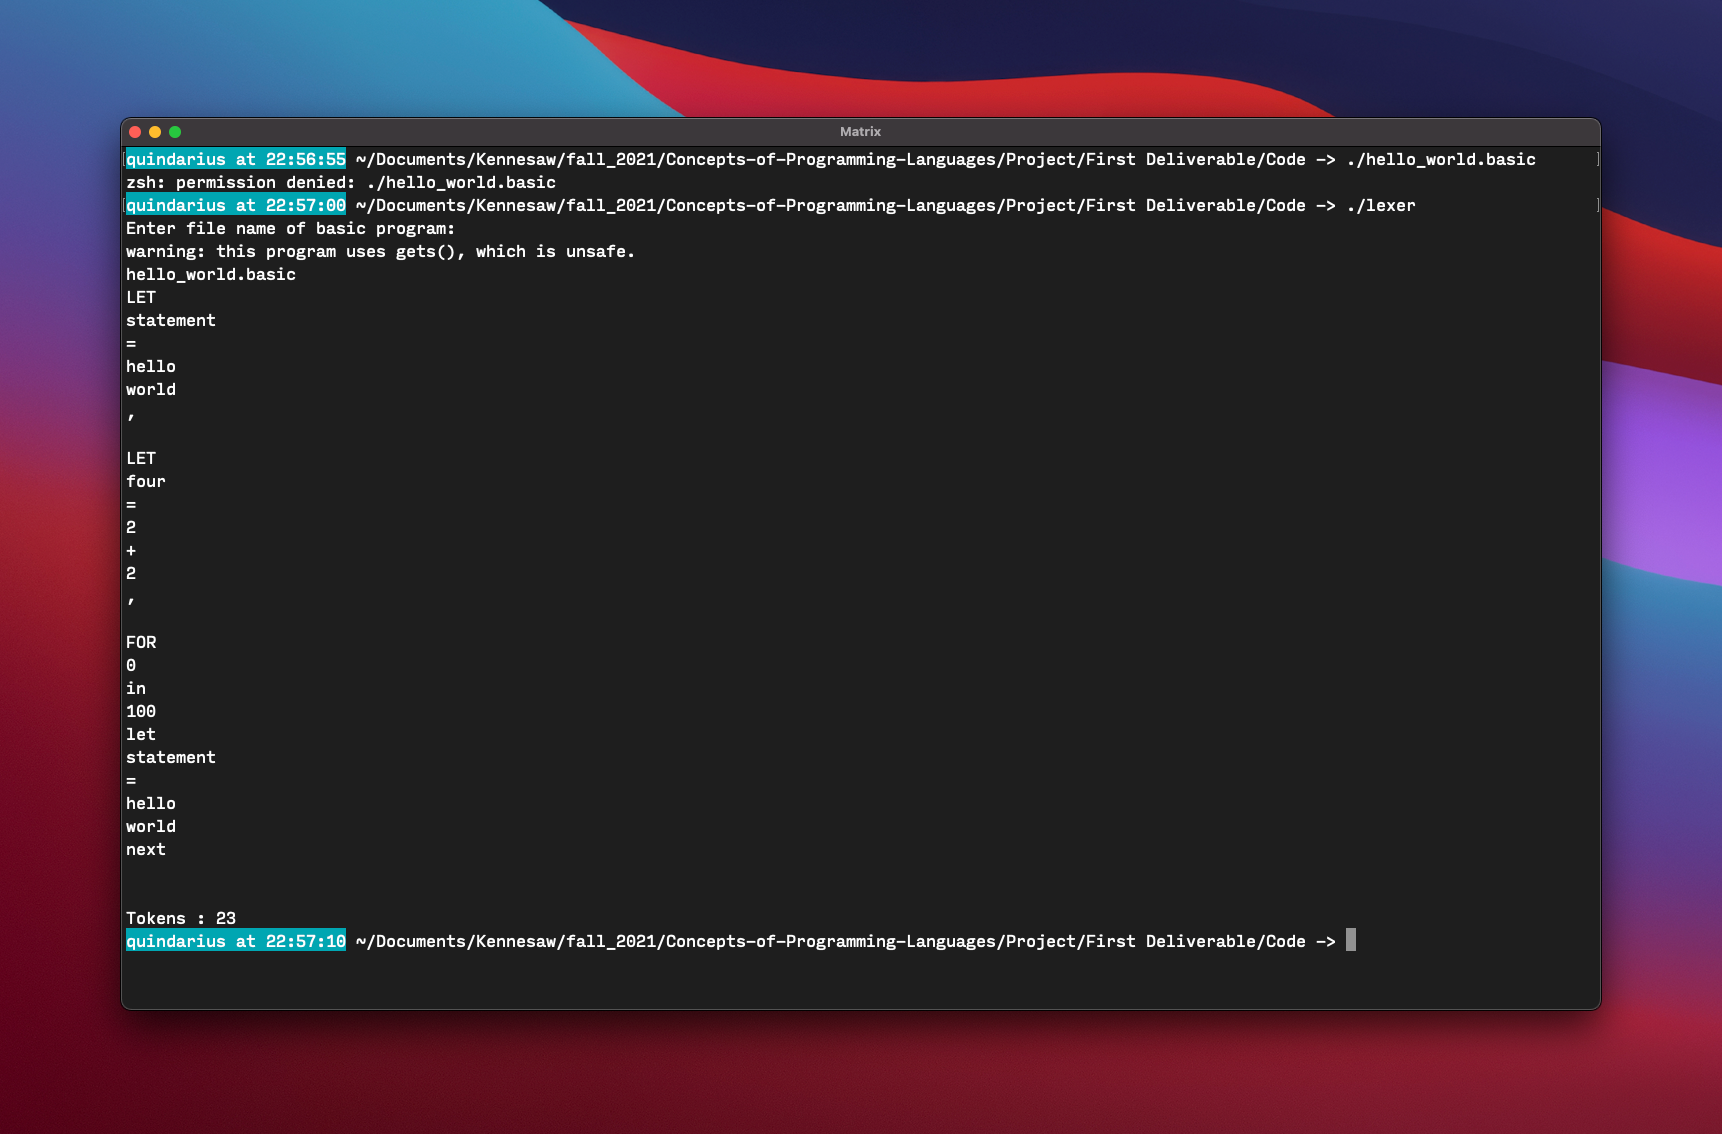
\includegraphics[width =\textwidth]{output}

\section{Summary}
After finishing this project I have learned what it takes to build a simple lexer(Scanner) for a language. 
This feels very incomplete but I know that it is only on piece out of many when it comes to building an intepreter. 
I am glad I kept the subset super small since working by myself I could make the project a little more approachable and actually used the free mind space to make the lexer in C so I could use a very portable language that someday in the future might come in handy. 
I can see where this work will also help me in my Natural Language Processing class. 
stripping text of tokens is such a huge part of the field and I was glad to be able to do this in C because when working with large amounts of data you would probably want to use a fast language. 
C fills this requirement but now I need to do my part and learn how to optimize the program. 
\end{document}

